\section[MIDI: An Introduction]{MIDI}\label{section:midi}

\subsection[What is MIDI?]{What is MIDI?}\label{section:what-midi}
The Musical Instrument Digital Interface (more commonly known as MIDI) is a digital communications protocol which allows for multiple hardware and software electronic instruments, controllers, computers, and related devices to communicate over a connected network\cite{Huber_2012}. It is used most to translate performance \say{events} (or musical notes) into its equivalent digital message, and then transmit these messages to other MIDI devices. These devices (MIDI receivers) can control sound generators or performance generators to create or modify music. Any MIDI-compatible device can send or receive MIDI messages from a MIDI controller (or the device sending the MIDI messages), and this will include all types of synthesizers. As an \say{interface,} MIDI is composed of a data communications link, and a system of hardware and software connected through this MIDI network. With MIDI, any electronic instruments and devices which are within a network can be worked with, through the transmission of a real-time performance and MIDI messages. These transmissions of performances and messages can then be put through the system to various instruments and devices through one singular data line, rather than multiple data streams, as this system can be chained from one device to another. A single data cable used with MIDI is capable of transmitting a real-time performance and MIDI-control message over 16 distinct channels, numbered appropriately one through sixteen. The musician working with the system will determine which of these channels to send information through, depending on which MIDI devices are being used\cite{Romano_2003}.

However, there are several limitations to the MIDI protocol. The first, and most important, limitation of MIDI is that it does not support sound. It is unable to communicate audio itself, or create sounds\cite{Huber_2012}. Instead, as a digital language, it instructs a compatible device or program to create, playback, or modify sounds. It will communicate an on/off status of a sound trigger, along with a range of parameters which instructs a MIDI receiver to control specified audio-related functions \cite{Kirk_Hunt_2013}. So, the data pathways for MIDI and audio routing will be different, even if they share a physical transmission cable, as in Figure \ref{fig:midi-system-with-audio-connections}\cite{Huber_2012}. 

\begin{figure}
	\centering
	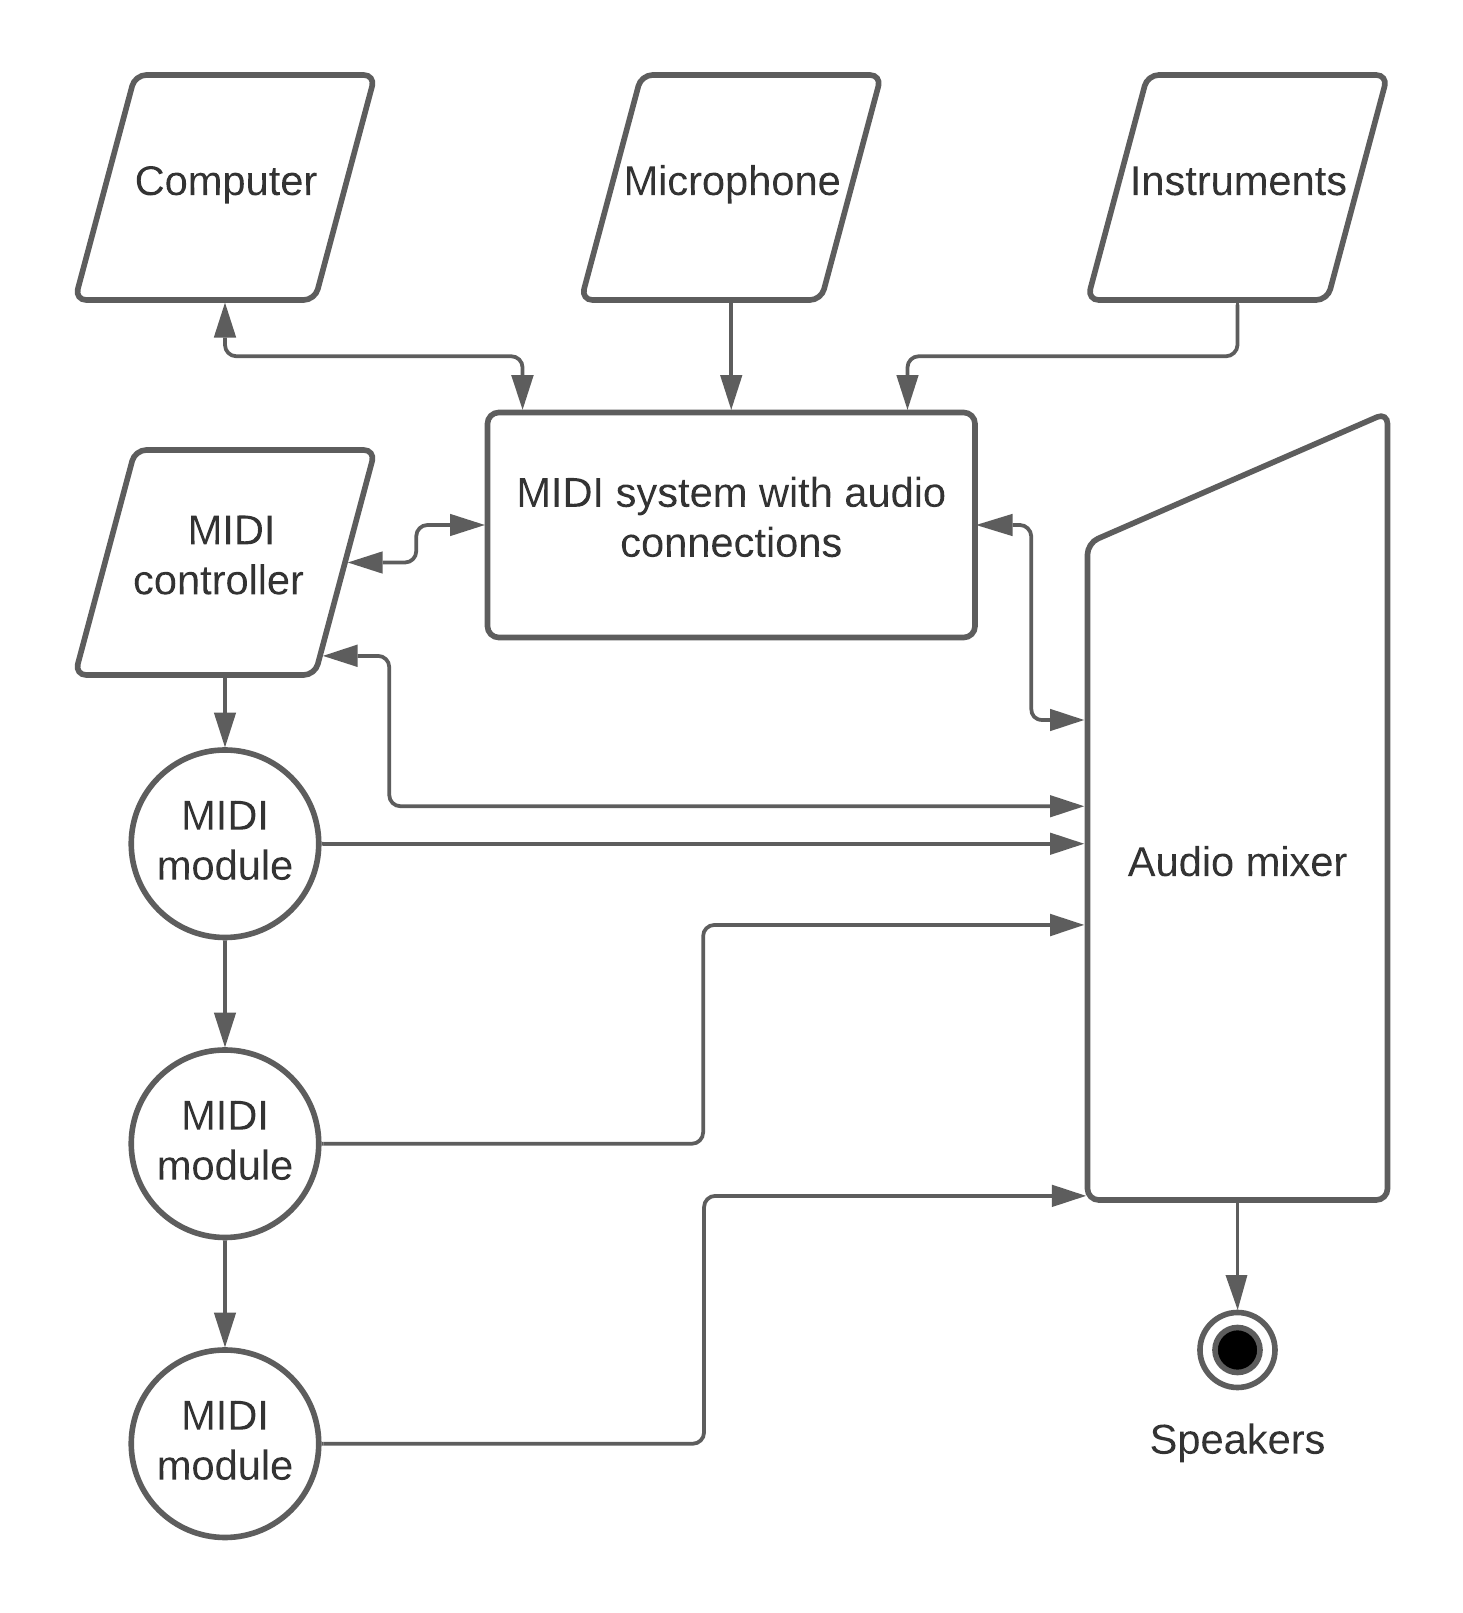
\includegraphics[width=0.35\textwidth]{figures/midi-system-with-audio-connections.png}
	\caption{The MIDI system, with audio connections}
	\label{fig:midi-system-with-audio-connections}
\end{figure}

Additionally, much of MIDI is built around the concept of keyboard notes and pitches. MIDI messages are primarily transmitted through the use of an electronic keyboard. So, for other types of MIDI instruments (such as a violin, or clarinet), there is a restriction to how a note may sound using MIDI. Certain characteristics of non-keyboard instruments (such as the ability of playing discrete semitone pitches\footnote{A discrete semitone pitch is another way of describing one pitch of the twelve-octave equal temperament tuning system.}) are more easily lost. For players of acoustic instruments, these issues are even more clear. Within MIDI, the velocity is considered to be a single note-on velocity, defining the dynamic response of the note to one value. For players of acoustic instruments, the velocity, or dynamic response, of a singular note is shaped by the player, along with the note's timbre and pitch when played\cite{Kirk_Hunt_2013}.

\subsection[How does MIDI work?]{How does MIDI work?}\label{subsection:how-midi}
From a hardware perspective, the MIDI protocol will determine which types of plugs can be used for MIDI connections. There are three possible \say{sockets} that can be used on any MIDI-compatible device:

\begin{enumerate}
	\item MIDI OUT: this will send data to other devices (MIDI receivers). An example of this will include an electronic keyboard which plays a note, and then \say{note messages} are sent out from the MIDI OUT socket.
	\item MIDI IN: this socket will receive the MIDI information from other devices. Using the previous example, if a keyboard's MIDI OUT socket is connected with a MIDI cable to another sound module's IN socket, then the sound module will be able to produce sound on behalf of the keyboard.
	\item MIDI THRU: this socket will relay the messages received at the MIDI IN socket, so more devices will be able to be chained together.
\end{enumerate}\label{enu:list-of-midi-sockets}

\begin{figure}
	\centering
	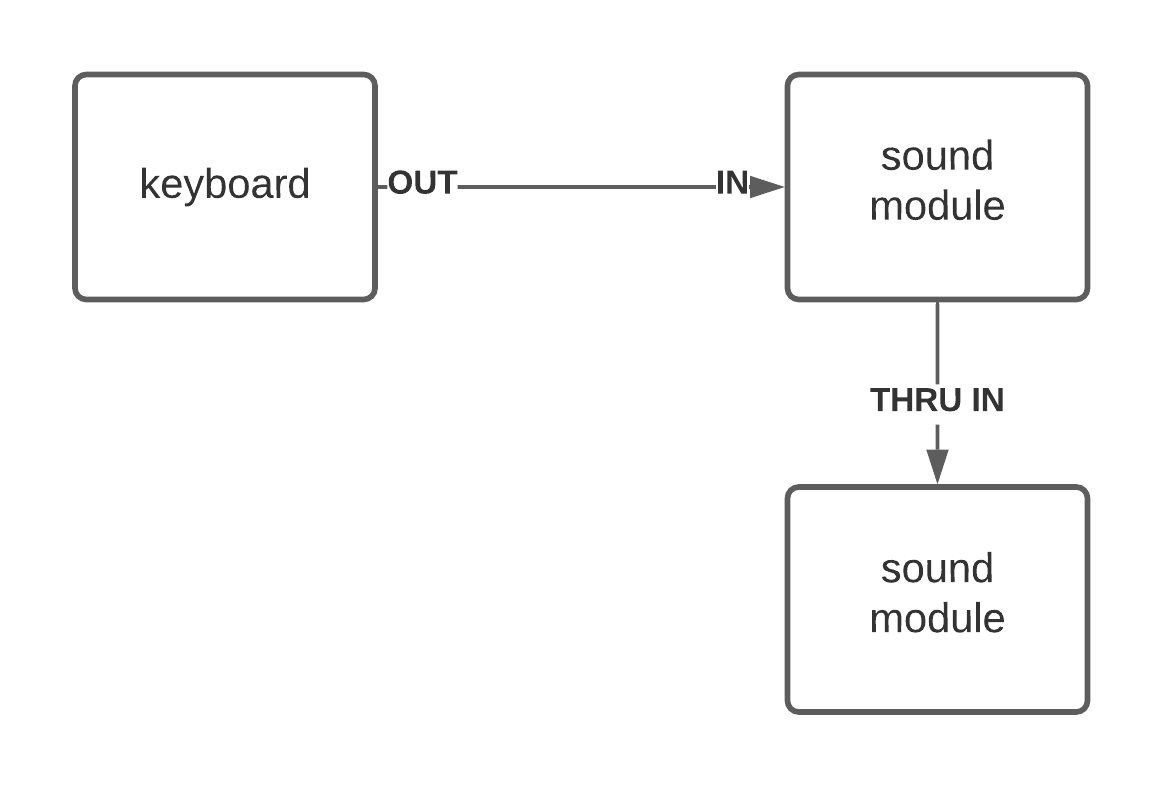
\includegraphics[width=0.5\textwidth]{figures/midi-sockets.png}
	\caption{MIDI sockets using an electronic keyboard}
	\label{fig:midi-sockets}
\end{figure}

Typically, this will result in the flow in Figure \ref{fig:midi-sockets}, as it is normal for a keyboard's OUT port to be connected to a sound module's IN port. This IN socket will then be connected to another sound module, through the THRU IN port of the first sound module, into the IN port of the second sound module. Thus, both modules are now driven by the keyboard\cite{Kirk_Hunt_2013}.

In a software view of the protocol, there are two basic types of messages MIDI is able to send: a \textit{channel} message, and a \textit{system} message. Channel messages are much more common. As previously mentioned, MIDI allows for the use of up to 16 different sounds to be controlled at the same time, through the use of its 16 different channels. So, each sound that must be played concurrently will be placed into a different \textit{MIDI channel}. Within the channel, there are seven distinct messages, each of which contain a specific meaning and role. The first is the \say{Note on} message. This is the most common MIDI message used, and is sent whenever a note on a MIDI controller is played or pressed down, most common as pressing a key on a keyboard. The data contained in this message will tell a sound module how hard and fast a note was played (the \textit{velocity} of a note), as well as which channel the note was played on\cite{Romano_2003}. The pitch of the message represents which key was pressed, and is defined as the number for each semitone on a keyboard. The semitone is the smallest interval of the modern Western tonal system. In equal temperament\footnote{Equal temperament is regarded to be the normal tuning of the West, a 12-note chromatic scale. This is also known as A440, in which the note $A_4$ is tuned relative to the standard pitch of 440Hz, and other notes are tuned as a specific number of semitones from this pitch.}--a tuning of the scale, based on a cycle of 12 identical fifths, and with the octave divided into 12 equal semitones--a semitone is the $\frac{1}{12}$ part of an octave. The notational system (i.e. sheet music) allows for three types of semitones to be distinguished: the diatonic, or the minor second (e.g. E-F, or C\musSharp{}-D), the chromatic, the difference between a major second and a minor second (e.g. F-F\musSharp{}, or D\musFlat{}-D), and the enharmonic, the doubly diminished third (e.g. G\musFlat{}\musFlat{}-E) \cite{Drabkin_Lindley_2001}. Middle C ($C_4$) is number 60 on the keyboard, and each semitone above and below Middle C is incremented or decremented accordingly\cite{Kirk_Hunt_2013}. 

The second is the \say{Note off} message, which turns off a note, or notes when a note is stopped. Like with Note on, Note off also contains values for channel, pitch, and velocity. For this message, only velocity's definition is changed, referring instead to the speed at which a note is released. The final common type of channel MIDI message is the \say{Pitch-bend,} which for electronic keyboard appears in the form of a physical wheel or sideways-moving handle of some type. Like its name implies, users will use this wheel or module to bend the pitch of notes currently being played. If the module is a physical wheel, it will return to its default position of zero (not bending a note) when the player lets go of the wheel. The pitch-bend will contain two pieces of data: the channel, and the pitch bend value. This value ranges from 0-127, with a value of 0 representing that the pitch has a full downwards bend to it, while a value of 127 represents the opposite, with a full upwards bend\cite{Kirk_Hunt_2013}. For this module, the value 64 will roughly indicate the center position on the wheel, and represent that a pitch has no bend applied to it.

MIDI also contains \say{system} messages, sent to all devices within the MIDI system\cite{Romano_2003}. These messages are not limited to a specified number of channels, and allow for a greater variety of data to be sent. There are three basic types of system messages\cite{Kirk_Hunt_2013}:

\begin{enumerate}
	\item real-time: this type of message allows the devices within the MIDI system to synchronize together.
	\item common: this message allows the devices to agree on some type of common musical issues, with tuning and song selection as two examples.
	\item exclusive: this message will exclusively send data to one device type. For manufacturers, these messages are used to send data to only one type of synthesizer or device type, serving as \say{add-ons} to MIDI.
\end{enumerate}\label{enu:midi-system-messages}

\noindent System messages are much harder to understand than channel messages, and so will not be discussed to great detail within the scope of this project.

\subsection[Constructing MIDI Messages]{Constructing MIDI Messages}\label{section:midi-messages}

MIDI messages are composed of three bytes, with a byte defined as a fundamental computation building block which consists of eight binary digits (or bits), either zero or one. Bytes which begin with a zero will be a \say{data byte} and bytes which begin with a one are \say{status bytes.} The most significant bit (MSB, or the leftmost binary bit within a MIDI message) is used to identity the byte type. The MSB of a data byte is 0, while the MSB of a status byte is 1.

\[\textrm{a status byte: } \textit{1xxx nnnn} \] \[\textrm{a data byte: } \textit{0nnn nnnn} \]

A status byte determines the type of MIDI function that will be performed, and encodes channel data, allowing the instruction to be received by a device that is set to respond to the selected channel. A data byte is used to associate a certain value to the event that is given by the accompanying status byte. This will determine the type of message that is sent (as they are normally channel messages) between note on, note off, pitch bend, or another type of message.

% TODO: this is confusing 
After the top bit/MSB of one in a status byte, which begins a MIDI message, the next three bits, or digits, are the bits which actively determine the type of message it is, of which there are eight possible combinations:

\[000, 001, 010, 100, 101, 110, 111 \]

The last four bits of a MIDI message determine which channel the message is delivered through, with 16 combinations for each of the 16 channels, as seen below. %TODO: fix the tables, so this makes sense

% TODO: have better transition between last section to talking about individual message types
\subsubsection{Note On Messages}

The note on message indicates the beginning of a MIDI note. Typically, one note on message is generated each time a note is triggered on a MIDI device, such as a keyboard, controller, or other MIDI instrument\footnote{This includes, pressing down a key, hitting a MIDI drum pad, or playing a MIDI sequence.}. A note on message will contain three bytes of information: the MIDI channel number, the pitch number, and the attack velocity value. As in Table \ref{tbl:byte-structure-note-on}, the first byte specifies that this MIDI message is a note on message, and the MIDI channel that this message will go through. The second byte determines the specific note, of the possible 128 notes numbered 0-127, which will be sounded by the MIDI instrument. The third and final byte of a note on message is the note's velocity, also ranged from 0-127. This will denote the loudness of the sounding note, increasing in volume the higher this value goes. For MIDI instruments which do no interpret the entire 128-numbered range of velocity values, we will instead see an attack velocity value of 64 used, regardless of how loud or soft the note itself may be played. This value of 64 gives the note a dynamic/loudness of \textit{mezzo forte}, or moderately loud. Additionally, a note on message with an attack velocity of 0 will generally be equivalent to a note off message, discussed in the next section. In a note on message with an attack velocity value of 0, the MIDI receiver will generally silence the currently-sounding note, by playing it with a velocity (or volume) value of 0\cite{Huber_2012}.

\begin{table}
	\centering
	\begin{tabular}{|c|c|c|}
	\hline
		Channel number (0-15) & Note number (0-127) & Attack velocity (0-127) \\
		\hline
		(1001 CCCC) & (0NNN NNNN) & (0VVV VVVV) \\
	\hline
	\end{tabular}
	\caption{The structure of a note on MIDI message}
	\label{tbl:byte-structure-note-on}
\end{table}

\subsubsection{Note Off Messages}

\begin{table}
	\centering
	\begin{tabular}{|c|c|c|}
	\hline
		Channel number (0-15) & Note number (0-127) & Release velocity (0-127) \\
		\hline
		(1001 CCCC) & (0NNN NNNN) & (0VVV VVVV) \\
	\hline
	\end{tabular}
	\caption{The structure of a note off MIDI message}
	\label{tbl:byte-structure-note-off}
\end{table}

A note off message is similar to that of a note on message, except that it is a command used to stop playing a MIDI note. A MIDI note on message will play until a corresponding note off message for that note is received by the MIDI receiver. So, a musical composition can, in its most basic form, be written as various MIDI note on and note off messages. There are also three bytes in a MIDI note off message (refer to table \ref{Tbl:byte-structure-note-off}), except that the third byte instead is a release velocity value. This value, also ranging from 0-127, will indicate the velocity in which a key or controller is released. A lower value indicates that the key was released slowly, and a higher value shows the key was released quickly. For MIDI devices which are able to respond to receiving a release velocity value, these are able to be programmed to vary the note's speed of decay, reducing the note's decay time as the release velocity value increases\cite{Kirk_Hunt_2013}. %TODO: explain what MIDI decay is

\subsubsection{Pressure/Aftertouch Messages}

\begin{table}
	\centering
	\begin{tabular}{|c|c|c|}
	\hline
		Channel number (0-15) & Note number (0-127) & Release velocity (0-127) \\
		\hline
		(1000 CCCC) & (0NNN NNNN) & (0VVV VVVV) \\
	\hline
	\end{tabular}
	\caption{The structure of an aftertouch MIDI message}
	\label{tbl:byte-structure-aftertouch}
\end{table}

Pressure messages, also known as \say{Aftertouch} messages, happen after a key is pressed, and the user decides to press down on the key harder. For compatible MIDI devices, aftertouch can generally be assigned to parameters which include vibrato, volume, filter cutoff, and pitch. As defined by MIDI, and the byte structure of an aftertouch message in Table \ref{tbl:byte-structure-aftertouch}, there are two types of aftertouch messages: channel pressure messages and polyphonic key pressure messages\cite{Huber_2012}. %TODO: define all the music terms

\begin{table}
	\centering
	\begin{tabular}{|c|c|c|}
	\hline
		Channel number (0-15) & Note number (0-127) & Pressure value (0-127) \\
		\hline
		(1101 CCCC) & (0NNN NNNN) & (0VVV VVVV) \\
	\hline
	\end{tabular}
	\caption{The structure of a channel pressure MIDI message}
	\label{tbl:byte-structure-channel-pressure-messages}
\end{table}

Channel pressure messages are messages commonly transmitted by instruments which only respond to a singular overall pressure, regardless of the total number of keys played. These messages also contain three bytes of information: the MIDI channel number, the note number, and pressure value, as in table \ref{Tbl:byte-structure-channel-pressure-messages}\cite{Huber_2012}. 

Polyphonic key pressure messages are similar to channel pressure messages, but respond to the pressure changes that are applied to the individual keys of a MIDI keyboard. A MIDI device compatible with this type of MIDI message is able to respond or transmit the individual key pressure messages of each key that is pressed down. How a MIDI device compatible with polyphonic key pressure messages will vary, but typically contain bindings for performance parameters which include vibrato, volume, timbre, and pitch\cite{McGuire_2014}. %TODO: this last sentence doesn't make 100% sense, make better -> define timbre

\subsubsection{Program Change Messages}

\begin{table}
	\centering
	\begin{tabular}{|c|c|}
	\hline
		Channel number (0-15) & Program ID number (0-127) \\
		\hline
		(1100 CCCC) & (0PPP PPPP) \\
	\hline
	\end{tabular}
	\caption{The structure of a program change message}
	\label{tbl:byte-structure-program-change}
\end{table}

Program Change messages are used to change the active program or preset number of a MIDI device. This preset number is a user- or factory-defined number to select a specific sound patch or system setup, to alter the output sound. With this message, up to 128 presets (in accordance to the established 0-127 numbered range available in MIDI) can be selected as a preset\cite{Huber_2012}. Commonly used to switch between presets on a digitally controlled mixing console, change loaded sounds, and more, this message consists of two bytes of information: the MIDI channel number, and the program ID number (0-127), like in Table \ref{tbl:byte-structure-program-change}.


\subsubsection{Pitch Bend Messages}

The pitch wheel is a common module found on most electronic keyboards and MIDI keyboards. The sensitivity of a pitch bend message refers to the responsiveness level (in semitones) of a pitch bend wheel or other pitch bend controller. This message is encoded in two bytes\cite{McGuire_2014}, and yields a total of 16,384 distinct semitone steps to pitch bend. Thus, the range of this message extends from its bottom end of -8192 to +8192, with 0 at the center serving as the instrument's true unaltered pitch\cite{Huber_2012}. This gives the physical pitch bend wheel values between 0 and 127, with 64 as the middle true pitch, as possible value ranges.

\subsubsection{Control Change Messages}

The control change type of MIDI message is typically referred to as a performance controller, as it is capable of communicating with the many knobs and sliders on MIDI controllers. These messages relate the real-time control over these performance parameters. There are three main types of control change messages:

\begin{enumerate}
	\item continuous controllers: controllers which relay a full range (0-127) of variable control settings.
	\item switch controllers: controllers which have an \say{off} and \say{on} state, with no intermediate settings.
	\item channel mode message controllers: controllers which range from the controller numbers 120 and 127, used to set the note's sounding status, the instrument reset, the local control's on/off, all notes off message, and the MIDI mode status of a device.
\end{enumerate}

\begin{table}
	\centering
	\begin{tabular}{|c|c|c|}
	\hline
		Channel number (0-15) & Controller ID number (0-127) & Corresponding controller value (0-127) \\
		\hline
		(1011 CCCC) & (0CCC CCCC) & (0VVV VVVV) \\
	\hline
	\end{tabular}
	\caption{The structure of a program change message}
	\label{tbl:byte-structure-control-change-message}
\end{table}

A control change message will be transmitted whenever the corresponding controllers are varied in real time \cite{Huber_2012}, and consist of three bytes: the MIDI channel number, controller ID number (0-127), and the corresponding controller value (0-127), as in table \ref{tbl:byte-structure-control-change-message}. The second byte of a control change message, which dictates the controller ID number, is used to specify which of the device's program or performance parameters are to be referenced. 

The third byte of the control change message, the controller value, describes the controller itself's actual data value. This is used to specify the position, depth, and/or level of a particular parameter\cite{Huber_2012}.